\section{Triple Context}\label{sec:pre}
%In this section, we introduce our model that learns embeddings of entities and relations with the help of triple context in the knowledge graph.
Firstly, we introduce some notations that are used in this paper. Let $\mathcal{K}$ be a knowledge graph, $\mathcal{E}$ and $\mathcal{R}$ the set of all entities and relations respectively in $\mathcal{K}$. Each triple is denoted as $(h, r, t)$, in which $h$ is the head entity, $t$ is the tail entity and $r$ is the relation between $h$ and $t$. The embeddings of each entity and relation are denoted in bold, e.g., $\bm{\mathrm{h}}$ is the embedding of $h$. All the embeddings are in $d$-dimensional space $\mathbb{R}^d$. Our goal is to learn embeddings of all entities and relations, which is denoted as $\Theta$. In the following subsections, we define neighbor context and path context, and then give the framework of our model.

\subsection{Neighbor Context}
Neighbor context of an entity is the surroundings of it in KG. It is the local structure that interacts most with the entity and can reflect various aspects of the entity. Specifically, given an entity $e$, the neighbor context of $e$ is a set $C_N(e)=\{(r,t)|\forall r, t, (e,r,t)\in\mathcal{K}\}$, where $r$ is an outgoing edge (relation) from $e$ and $t$ is the entity it reaches through $r$. In other words, the neighbor context of $e$ is all the \textit{relation-tail} pairs appearing in triples with $e$ as the head. For example, as shown in Figure~\ref{pic1}, the neighbor context of entity $h$ is $C_N(h)=\{(r_4, e_1), (r_3, e_2), (r_2, e_3), (r_1, e_8), (r_1, e_{10})\}$. We predict the appearance of an entity based on its neighbor context in our model, as a measurement of the compatibility of the entity and its neighbor context.

\begin{figure}
  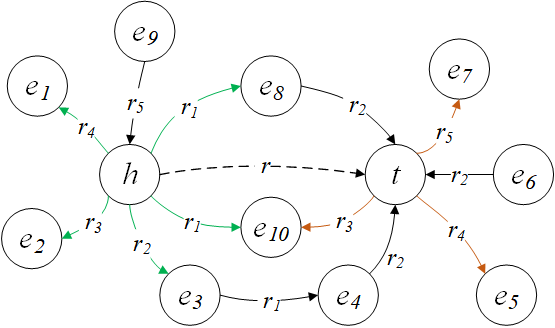
\includegraphics[width=0.45\textwidth]{pic1.png}
  \caption{An illustration of the \emph{triple context} of a triple $(h,r,t)$ in a knowledge graph.}
  \label{pic1}
\end{figure}


\subsection{Path Context}
Path context of a pair of entities is the set of paths that starts from an entity to the other in a KG. It is helpful in modeling the relation and capturing interactions between the pair of entities. Given a pair of entities $(h,t)$, the path context of $(h,t)$ is a set $C_P(h,t)=\{p_i | \forall r_{m_1}, \cdots, r_{m_i}, e_1, \cdots, e_{m_i-1},$ $p_i=(r_{m_1}, \cdots, r_{m_i}), (h,r_{m_1},e_1)\in\mathcal{K}, \cdots, (e_{m_i-1}, r_{m_i}, t)\in\mathcal{K}\}$, where $p_i=$ is a list of relations (labeled edges) through which it can traverse from $h$ to $t$, $m_i$ is the length of path $p_i$. In Figure~\ref{pic1}, the path context between $h$ and $t$ is $C_P(h,t) = \{(r_1, r_2), (r_2, r_1, r_2)\}$. We use the path context to predict the tail entity of a triple given the head entity.
